\documentclass[10pt,conference]{IEEEtran}
\IEEEoverridecommandlockouts
% The preceding line is only needed to identify funding in the first footnote. If that is unneeded, please comment it out.
\usepackage{cite}
\usepackage{amsmath,amssymb,amsfonts}
\usepackage{algorithmic}
\usepackage{graphicx}
\usepackage{textcomp}
\usepackage{xcolor}
\usepackage{makecell}
\usepackage{appendix}
\usepackage[margin=1in]{geometry}
\renewcommand{\baselinestretch}{1}
\def\BibTeX{{\rm B\kern-.05em{\sc i\kern-.025em b}\kern-.08em
    T\kern-.1667em\lower.7ex\hbox{E}\kern-.125emX}}
\begin{document}

\title{Cyberbullying Detection using ML: A comparative study between supervised and semi-supervised methods

}

\author{\IEEEauthorblockN{Dev Kathuria}
\IEEEauthorblockA{\textit{Computer Science Engineering Student} \\
\textit{Shiv Nadar University}\\
email: dk382@snu.edu.in}

}

\maketitle

\begin{abstract}
Bullying has been prevalent since the beginning of time, It’s just the ways of bullying which have changed over the years, from physical bullying to cyberbullying. According to Williard(2004), there are eight types of cyberbullying such as harassment, denigration, impersonation, etc. It’s been around 2 decades since social media sites came into the picture, but there hasn’t been a lot of effective measures to curb social bullying and it has become one of the alarming issues in recent times.  This paper does a comparative study of various Supervised and semi-supervised learning algorithms. The evaluation of the result shows that Ensemble supervised methods perform better than traditional supervised methods and the semi-supervised methods as well.

\end{abstract}

\begin{IEEEkeywords}
Machine Learning, Cyberbullying, Supervised, Semi-supervised, Detection, Ensemble
\end{IEEEkeywords}

\section{DATA}
This section contains all the aspects of Data from collection to preprocessing and features extraction.

\subsection{Data Collection}

I have used a combination of two datasets to arrive at the final results, Initial plan was to use just the first dataset[1], which didn’t give good results[refer Appendix \ref{appendices:Appendix A} for details], So I decided to merge the two datasets, where the second dataset had a high percentage of cyberbullying instances.

Here is the Detailed Description of both the datasets.
\begin{enumerate}

    \item Formspring Data for CyberBullying \cite{b1}
    \begin{enumerate}
        \item
        Data crawled from Formspring.me, crawled in 2010, manually labelled by Amazon’s Mechanical Turk
        
        \begin{table}[htbp]
        \caption{3 occurrences of labelled formspring data}
        \begin{center}
        
        \begin{tabular}{|c|c|c|}
            \hline
              ANSWER & \makecell{Yes or No whether \\ it contains
              cyberbullying or not} \\
             \hline
             CYBERBULLYINGWORK & \makecell{ Phrase(s) or word(s)  identified \\ by the worker which corresponds \\ to  cyberbullying} \\
             \hline
             SEVERITY & 0(NO Bullying) to 10 \\
             \hline
            
        \end{tabular}
        \end{center}
        \end{table}
        
        
        \item
        Total Instances: 12852  
      \end{enumerate}
    \item Dataset for Detection of Cyber-Trolls \cite{b2}
    \begin{enumerate}
        \item It is a partially manually labelled dataset.
        \item Total Instances: 20001
        
The dataset just has 2 attributes- tweet and label[0 corresponds to No while 1 corresponds to Yes]
    \end{enumerate}
\end{enumerate}
\subsection{Data Cleaning}
All the datasets were in CSV format and they had to be converted to ARFF, so that it could be used by Weka to run various ML classifiers, sadly integrated 'CSV to ARFF weka converter' and the online CSV to ARFF converters gave a lot of errors, so it had to be done manually.

I have advance experience in working with Excel, so I’ve used it for basic data cleaning and then using 'ATOM text editor', I added all the attribute relation and renamed it as a 'ARFF' file.

Various steps performed using Excel:

\begin{enumerate}
    \item Used inbuilt excel command “clean()” to remove any non-printable characters
    \item Used “IsBlank()” to search for any missing records and deleted any row which had any missing value
    \item For ARFF format, all the text had to be converted to a string, I did that using format cell options by using a custom processor (\textbackslash{}\textquotedblright{}@\textbackslash{}\textquotedblright{})
    \item Any extra newline character had to be removed, which was done using find and replace by using ASCII code for a line character. Moreover any extra characters which were easily noticeable such as 'Q:', 'A:',' \textless br\textgreater ','@quot' etc were removed in the same way
    \item using hit and trial, multiple other errors producing elements were later removed
    

\end{enumerate}

\begin{table}[htbp]
    \caption{Instances}
    \centering
    \begin{tabular}{|c|c|c|c|}
        \hline
         & \textbf{Formspring} & \textbf{Twitter} & \textbf{Merged} \\
         \hline
        Total Instances & 10928 & 10708 & 19752 \\
        \hline
        CB instances & 220 & 2505 & 2725 \\
        \hline
        Non-CB instances & 10928 & 6312 & 17027\\ 
        \hline
    \end{tabular}
    \label{tab:my_label}
\end{table}

\subsection{Data Preprocessing}
Since after manually converting data into ARFF format, I applied NumerictoNominal filter on our class to convert it to nominal, then the preprocessing steps were done as follows using the unsupervised StringtoVector filter[check Screenshot-preprocess filter  for detailed configuration]:
\begin{enumerate}
    \item Word Tokenization, It converts our text to separate words in a list, in which I used certain extra delimiters  \{ , ; : ' \textquotedblright{} ( ) ? ! / - \_ \textgreater{} \textless{} \& \# 1 2 3 4 5 6 7 8 9 0 \} 
    after going through the data, I also filtered out any numeric content as it doesn’t contribute to cyberbullying.
    \item Lowering Text using Lower case only tokens setting on Weka
    \item Stop words and encoding cleaning using Weka’s MultistopWords Algorithm
    \item Stemming: Initially I didn’t do stemming which produced bad results, after evaluating “CfsSubset Eval” and “InfoGainAttributeEval using Ranker for searching”[Appendix \ref{appendices: Appendix B}], I used “Lovins Stemmer” for the same
    \item Now after manually going through the attributes, all the unnecessary attributes which weren’t filtered  such as [\textdollar{},=d,=p,*] etc, were removed manually
    \item Now the next step was to extract features so that it can be used with ML algorithms, for which I used TF-IDF Transform using Weka. TF-IDF is a statistical measure to evaluate the relevance of a word, which is basically calculated by multiplying the number of times that words appeared in the document by the inverse document frequency of the word

\end{enumerate}

\subsection{Data Resampling}
As the data was skewed, Resampling had to be performed on the training data, Firstly the data was split into Training and Test in 70:30 ratio and resampling was performed on the training data. Note: I did a slightly different kind of resampling for Supervised and semi-supervised learning(More details are given later).
\begin{table}[]
    \caption{Test and training Instances}
    \centering
    \begin{tabular}{|c|c|c|}
    \hline
         & Test & Training \\
    \hline
    Total Instance & 5926 & 13826 \\
    \hline
    CB Instances & 616 &1909 \\
    \hline
    Non-CB instances & 5110 & 11917 \\
    \hline
    \end{tabular}
    \label{tab:my_label}
\end{table}

\subsubsection{Supervised Learning}
\begin{itemize}
    \item As I had ample data to work with(using Merged dataset), I used Undersampling of majority class followed by oversampling of the minority class
    \item For Oversampling, Supervised Resample filter is used with a bias towards uniform class as 1(100\%) and noReplacement set as false
    \item For Undersampling, the same filter is used with noReplacement set as true
    \\
    
	After resampling, training data had 4411 CB \& NON-CB instances

\end{itemize}

\subsubsection{SemiSupervised Learning}
Since Semi-Supervised learning has to have an unlabelled dataset, along with test and training datasets, I decided to use the instances which were labelled as invalid during the cleaning for Formspring dataset (around 2000 instances) as the unlabelled dataset, since Weka’s collective semi-supervised framework still has a lot of bugs [Refer screenshot err,err2], I couldn’t use the separate unlabelled dataset. To tackle this problem, I used 10 fold cross-validation to estimate the model. It works by automatically dividing the datasets and computing the results for every fold, resulting in an averaged output.

Since we are using cross-validation, we have to carefully resample the data to prevent the model from showing false accuracy. Firstly, I computed the model using unsampled dataset and then I just undersampled the majority class till it was nearly balanced by repeatedly using the beforementioned undersampling filter.

Since Initially, the plan was to use it along with the unlabelled dataset, it had a few extra attributes(Total: 1509 attributes) as compared to the datasets used in supervised learning(Since those attributes have 0 weights in the training dataset, they don’t really matter and it is more or less similar to the dataset used in supervised learning)
\begin{table}[htbp]
    \caption{Semi-Supervised Learning dataset}
    \centering
    \begin{tabular}{|c|c|c|}
    \hline
         & NoSampling & Sampling \\
    \hline
    Total Instances & 13826 & 3844 \\
    \hline
    CB instances & 1883 & 1883 \\
    \hline
    Non-CB instances & 11943 & 1961 \\
    \hline

    \end{tabular}
    
    \label{tab:my_label}
\end{table}


\section{EXPERIMENTAL RESULTS}
For supervised learning, I’ve used NaiveBayes, SVM, J48, RandomForest and Ensemble methods- AdaBoost-NaiveBayes, AdaBoost-SVM, Bagging-j48. Where Naive Bayes Performed the poorest and RandomForest gave the best result in terms of every metric.[fig1 \& fig2]
For semisupervised learning, I’ve used YATSI and Collective IBk for unbalanced and balanced datasets, where the result of the unbalanced dataset came out to be bad as expected while the results of Unbalanced dataset are still considerable, giving an average accuracy of around 63.5\%, thus performing poorly in comparison to supervised methods

Metrics used are:
\begin{itemize}
    \item ROCArea, which denotes the area under the curve formed by plotting TP rate.
    \item\[F-Measure = \frac{(2 \times Precison \times Recall)}{Precision + Recall}\]

    \item \[Accuracy = \frac{TP+TN}{TP+TN+FP+FN}\]
    \item \[Precision = \frac{TP}{TP+FP}\]
    \item \[Recall = \frac{TP}{TP+FN}\]
\end{itemize}


\subsubsection{Supervised}
Traditional Supervised Learning used: NaiveBayes, SVM, J48, RandomForest

Ensemble Learning Methods used: AdaBoost-NaiveBayes, AdaBoost-SVM, Bagging-j48, 

Figure 1 and Figure 2 shows a graphical comparison between the aforementioned algorithms
\begin{table}[htbp]
\caption{Supervised Traditional Methods}
\centering
\begin{tabular}{lllll}
{\color[HTML]{000000} }          & {\color[HTML]{000000} NaiveBayes} & {\color[HTML]{000000} SVM}   & {\color[HTML]{000000} J48}   & {\color[HTML]{000000} RandomForest} \\
{\color[HTML]{000000} ROCArea}   & {\color[HTML]{000000} 0.693}      & {\color[HTML]{000000} 0.721} & {\color[HTML]{000000} 0.722} & {\color[HTML]{000000} 0.803}        \\
{\color[HTML]{000000} F-Measure} & {\color[HTML]{000000} 0.648}      & {\color[HTML]{000000} 0.763} & {\color[HTML]{000000} 0.775} & {\color[HTML]{000000} 0.809}        \\
{\color[HTML]{000000} Precision} & {\color[HTML]{000000} 0.827}      & {\color[HTML]{000000} 0.852} & {\color[HTML]{000000} 0.840} & {\color[HTML]{000000} 0.841}        \\
{\color[HTML]{000000} Recall}    & {\color[HTML]{000000} 0.584}      & {\color[HTML]{000000} 0.723} & {\color[HTML]{000000} 0.741} & {\color[HTML]{000000} 0.789}       
{\color[HTML]{000000} }                 & {\color[HTML]{000000} }                                                            & {\color[HTML]{000000} }                                                            & {\color[HTML]{000000} }                                                            & {\color[HTML]{000000} }                                                           \\
{\color[HTML]{000000} \makecell{Confusion \\
Matrix}} & {\color[HTML]{000000} \begin{tabular}[c]{@{}l@{}}2874 2236\\ 231 585\end{tabular}} & {\color[HTML]{000000} \begin{tabular}[c]{@{}l@{}}3699 1411\\ 230 586\end{tabular}} & {\color[HTML]{000000} \begin{tabular}[c]{@{}l@{}}3881 1229\\ 303 513\end{tabular}} & {\color[HTML]{000000} \begin{tabular}[c]{@{}l@{}}4221 889\\ 360 456\end{tabular}}

\end{tabular}
\end{table}

\begin{table}[htbp]
\caption{Supervised Ensemble Methods}
\centering
\begin{tabular}{llll}
{\color[HTML]{000000} }                 & {\color[HTML]{000000} AdaBoost-NB}                                                      & {\color[HTML]{000000} AdaBoost-SVM}                                                     & {\color[HTML]{000000} Bagging-J48}                                                     \\
{\color[HTML]{000000} ROCArea}          & {\color[HTML]{000000} 0.745}                                                       & {\color[HTML]{000000} 0.731}                                                       & {\color[HTML]{000000} 0.802}                                                       \\
{\color[HTML]{000000} F-Measure}        & {\color[HTML]{000000} 0.749}                                                       & {\color[HTML]{000000} 0.764}                                                       & {\color[HTML]{000000} 0.781}                                                       \\
{\color[HTML]{000000} Precision}        & {\color[HTML]{000000} 0.842}                                                       & {\color[HTML]{000000} 0.837}                                                       & {\color[HTML]{000000} 0.845}                                                       \\
{\color[HTML]{000000} Recall}           & {\color[HTML]{000000} 0.707}                                                       & {\color[HTML]{000000} 0.727}                                                       & {\color[HTML]{000000} 0.748}                                                       \\
                                       &                                                                                    &                                                                                    &                                                                                    \\
{\color[HTML]{000000} \makecell{Confusion \\ Matrix}} & {\color[HTML]{000000} \begin{tabular}[c]{@{}l@{}}3635 1475\\ 263 553\end{tabular}} & {\color[HTML]{000000} \begin{tabular}[c]{@{}l@{}}3793 1317\\ 302 514\end{tabular}} & {\color[HTML]{000000} \begin{tabular}[c]{@{}l@{}}3906 1204\\ 288 528\end{tabular}}
\end{tabular}
\end{table}
\begin{figure}[htbp]
\centerline{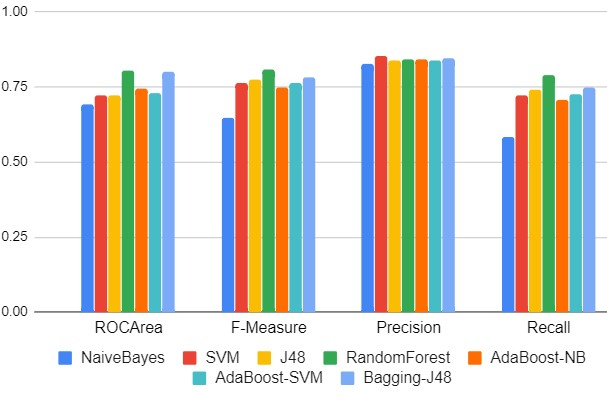
\includegraphics[width=8cm,height=10cm,keepaspectratio]{Screenshot_11.jpg}}
\caption{ROCArea, Fscore, Precision, Recall}
\label{fig}
\end{figure}

\begin{figure}[htbp]
\centerline{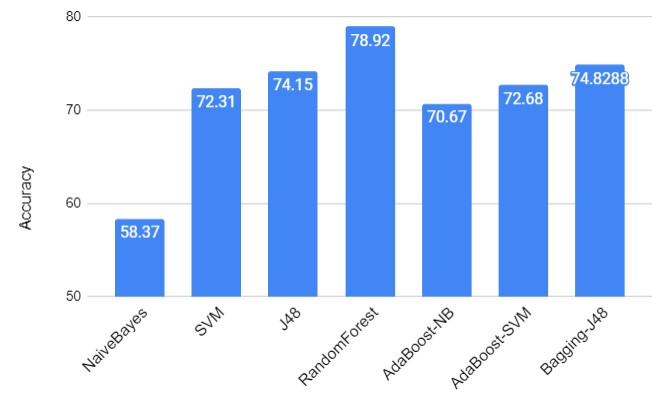
\includegraphics[width=9cm,height=10cm,keepaspectratio]{Screenshot_22.jpg}}
\caption{Accuracy}
\label{fig}
\end{figure}

\subsubsection{Semi-Supervised}
Algorithms Used:
\begin{enumerate}
    \item YATSI
    
    “Yet another Two-Stage Idea” is a collective classifier that uses the given classifier to train on the training set and labelling the unlabelled dataset, As a classifier, I chose J48 decision trees to generate a pruned or unpruned C4.5 decision tree. Predictions are then done by k nearest neighbours, for which I chose the KDTree search algorithm that uses Euclidean distance as a distance function. \cite{b3}
    \item Collective IBk
    
    \textit{It uses IBk to determine the optimal K for the neighbourhood on the training set. This K is used to build for each instance of the test set a neighbourhood, consisting of instances from the test AND training set.}
    
    \textit{Majority vote is used to determine the class label for an instance, based on its neighbourhood (in case of ties the first encountered class is taken). Sooner or later all labels of the test set are determined.}
    
    \textit{An instance that is presented for classification is then only looked up and the determined label is returned} \cite{b4}

\end{enumerate}



\begin{table}[]
\caption{Semi-Supervised Methods}
\begin{tabular}{lllll}
                                        & \multicolumn{2}{l}{{\color[HTML]{333333} \textbf{UNBALANCED}}}                                                                                                             & \multicolumn{2}{l}{{\color[HTML]{333333} \textbf{BALANCED}}}                                                                                                            \\
{\color[HTML]{000000} }                 & {\color[HTML]{3166FF} YATSI}                                                        & {\color[HTML]{FE0000} IBk}                                                           & {\color[HTML]{3531FF} YATSI}                                                       & {\color[HTML]{FE0000} IBk}                                                         \\
                                        & \multicolumn{2}{l}{{\color[HTML]{656565} \textit{\begin{tabular}[c]{@{}l@{}}(Weighted, average, \\ Value for CB class)\end{tabular}}}}                                     & \multicolumn{2}{l}{{\color[HTML]{656565} \textit{(Weighted Average)}}}                                                                                                  \\
{\color[HTML]{000000} ROCArea}          & {\color[HTML]{3166FF} 0.73, 0.73}                                                   & {\color[HTML]{FE0000} 0.59,0.59}                                                     & {\color[HTML]{3531FF} 0.676}                                                       & {\color[HTML]{FE0000} 0.653}                                                       \\
{\color[HTML]{000000} F-Measure}        & {\color[HTML]{3166FF} 0.82, 0.19}                                                   & {\color[HTML]{FE0000} 0.81,0.30}                                                     & {\color[HTML]{3531FF} 0.62}                                                        & {\color[HTML]{FE0000} 0.650}                                                       \\
{\color[HTML]{000000} Precision}        & {\color[HTML]{3166FF} 0.80, 0.36}                                                   & {\color[HTML]{FE0000} 0.81,0.31}                                                     & {\color[HTML]{3531FF} 0.62}                                                        & {\color[HTML]{FE0000} 0.657}                                                       \\
{\color[HTML]{000000} Recall}           & {\color[HTML]{3166FF} 0.85, 0.12}                                                   & {\color[HTML]{FE0000} 0.81,0.30}                                                     & {\color[HTML]{3531FF} 0.625}                                                       & {\color[HTML]{FE0000} 0.652}                                                       \\
{\color[HTML]{000000} Accuracy}         & {\color[HTML]{3166FF} 84.5}                                                         & {\color[HTML]{FE0000} 81.5}                                                          & {\color[HTML]{3531FF} 62.5}                                                        & {\color[HTML]{FE0000} 65.1}                                                        \\
\\
{\color[HTML]{000000} \makecell{Confusion \\ Matrix}} & {\color[HTML]{3166FF} \begin{tabular}[c]{@{}l@{}}11513 430\\ 1645 238\end{tabular}} & {\color[HTML]{FE0000} \begin{tabular}[c]{@{}l@{}}10685 1258\\ 1312 571\end{tabular}} & {\color[HTML]{3531FF} \begin{tabular}[c]{@{}l@{}}1132 829\\ 611 1272\end{tabular}} & {\color[HTML]{FE0000} \begin{tabular}[c]{@{}l@{}}1135 826\\ 512 1371\end{tabular}}
\end{tabular}
\end{table}
\begin{figure}
    \centering
    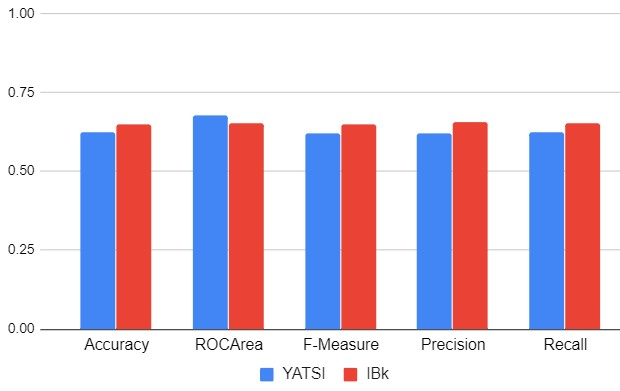
\includegraphics[width=8cm,height=10cm,keepaspectratio]{Screenshot_33.jpg}
    \caption{Yatsi and IBK on Balanced Dataset}
    \label{fig:my_label}
\end{figure}
Running the classifiers on the Unbalanced dataset gave dissatisfying results,  it looks like they have high accuracy, which is just a result of base rate fallacy, I’ve specifically mentioned individual scores for the Cyberbullying class for the unbalanced dataset in table VII so that it becomes clear that running the classifiers on unbalanced dataset gives a poor result, with high false-positive rate.

Running both the classifiers on the undersampled data, provided much better output, and since, the weighted average didn’t have a lot of deviation from the scores of either of the classes, I’ve just mentioned the weighted average scores for both of them
The average accuracy came out to be about 63\%, which in comparison to the Supervised algorithms is poor


\section{Related Work}
For Detecting Cyberbullying, numerous approaches have been developed, majorly using Natural Language Processing and Information Retrieval which are then used to classify textual data by extracting it's features by using TF-IDF, Sentiment Analysis, Dimensionality Reduction etc. and they have recieved commendable accuracies

Sambhagadi et al.\cite{b5} Detects nastiness using NLP techniques, they use a list of profanities as an extra feature along with analyzing the context as in which they are used, whether they are insulting or neutral in nature. They used modified linear SVM to classify the ASK.FM data, they even took the emojis into the picture. They got an F1 score of 0.59. 

Yao et al.\cite{b6} acknowledges the repetitive nature of cyberbullying on social media i.e a sequence of aggressive messages sent from bully to a victim with the intent of harm, previous paper, and multiple other papers used profanity to classify toxic comments as cyberbullying, disregarding its repetitive process. This paper uses sequential hypothesis testing formulation to drastically reduce the number of features used in classification, while still maintaining high accuracy.

Nandhini et al.\cite{b7} Proposes a naive Bayes based learning model and used the dataset of MySpace.com, they achieved a high accuracy of 91\%. \cite{b8} uses Formspring data, available at Kaggle.com by Kelly Reynolds which initially had about 12000 instances, but after preprocessing, they got a total of 1608 instances where half of them corresponds to cyberbullying, basically, they used this small dataset to train a Neural network and an SVM Classifier.

\begin{table}[htbp]
\caption{Results of \cite{b8} (in \%)}
\begin{tabular}{lllll}
Classifier     & \makecell{Average \\ Accuracy} & \makecell{Average \\ Recall} & \makecell{Average \\ Precision} & \makecell{Average \\ F-score} \\
\\
Neural Network & 91.76            & 91.7           & 92.4              & 91.9            \\
SVM            & 89.87            & 90.1           & 89.6              & 89.8           
\end{tabular}
\end{table}

\cite{b9} uses Logistic Regression and SVM to train on cyberbullying data

\begin{table}[htbp]
\caption{Results of \cite{b9} (in \%)}
\begin{tabular}{lllll}
Classifier     & \makecell{Average \\ Accuracy} & \makecell{Average \\ Recall} & \makecell{Average \\ Precision} & \makecell{Average \\ F-score} \\
\\
Logistic Regression & 73.76 & 61.47 & 64.4 & 62.9 \\
SVM            & 77.65 & 58.29 & 70.29 & 63.7 \\           
\end{tabular}
\end{table}

Study by Huang et al.\cite{b10} focuses on analyzing the social network structure between users and deriving features such as a number of friends, network embeddedness, and relationship centrality, by integrating textual features with social network features, detection of cyberbullying can be achieved. The study claims that past researches haven’t fully utilized social media features, this paper proposes cyberbullying detection beyond textual analysis to also consider the social relationships in which these bullying messages are exchanged. It uses twitter corpus and uses Weka 3.0 to implement it with different classification algorithms such as Naive Bayes, J48, SMO, Bagging and dagging.

\begin{table}[htbp]
\caption{Results of \cite{b10}}
\centering
\begin{tabular}{lll}
        & ROC & TP \\
       Bagging & 0.700 & 0.211\\
       J48 & 0.628 & 0.259\\
       SMO & 0.703 & 0.733 \\
       Dagging & 0.755 & 0.763 \\
       Naive Bayes & 0.695 & 0.723 
       
\end{tabular}
\end{table}
The results of this study is very much comparable to my work as well, as I got Similar values for those metric as well, Furthermore, Bagging using J48 as base and Supervised RandomForest algorithm got even better results than this.

The best result in \cite{b10} is recieved using Dagging, giving a ROC value of 0.755, which when compared to Bagging(ROC: 0.802) and RandomForest(ROC: 0.803) is less.

\cite{b11}, This paper uses Formspring dataset available on Kaggle, it trains classifiers and Neural networks, firstly on the Unbalanced Dataset and then on the Balanced Dataset, Similar to what I did for semi-supervised learning, This paper achieves the best result using Twitter Embeddings along with C-LSTM (Kim et al 2015) and achieves a Precision value of 0.485, Recall of 0.448 and F-measure of 0.444. It again obtains the best result using the same architecture on the balanced dataset:(Refer table X)


\begin{table}[htbp]
\caption{Results of \cite{b11} in comparison to Semi supervised Methods tested on Balanced Data in my paper}
\centering
\begin{tabular}{llll}
        & Precision & Recall & F-measure \\
        \\
       Rosa et al\cite{b11} & 0.845 & 0.842 & 0.842\\
       \\
       \makecell{Semi-supervised \\ (Balanced data)} & 0.62 & 0.625 & 0.62 \\
       
\end{tabular}
\end{table}

\section{Conclusion}
In this paper, I did a comparative study between various Supervised and semi-supervised algorithms, Additionally, I compared various Supervised Ensemble methods as well. The overall best performance was shown by RandomForest classifier, the Ensemble methods performed a tad bit worse than the best traditional Supervised method, but still, I observed a high True positive rate for the cyberbullying class in all the ensemble methods, which is much more desirable. NaiveBayes performed the worst, giving just 58\% accuracy.

I used 2 semi-supervised Learning algorithms with cross-validation on Balanced and Unbalanced datasets, Both of them performed much better on the Balanced dataset, giving approximately the same performance. Average accuracy for Semi-Supervised methods came out to be approximately 63.5\%, which is better than NaiveBayes but worse than all other tested algorithms

 In this paper, I evaluated my approach and compared it with other papers in the section “Related Work” I also observed that none of the studied past researches used any semi-supervised methods, probably because they are not that popular or effective as in our case they didn’t give any commendable result in comparison to the supervised methods.







\begin{thebibliography}{00}
\bibitem{b1} "Formspring Data for Cyberbullying Detection." Kaggle: Your Machine Learning and Data Science Community, www.kaggle.com/swetaagrawal/formspring-data-for-cyberbullying-detection. Accessed 19 Mar. 
\bibitem{b2} Dataturks – Online Tool to Build Image Bounding Box, NER, NLP and Other ML Datasets, dataturks.com/projects/abhishek.narayanan/Dataset\%20for\%20
Detection\%20of\%20Cyber-Trolls. 
\bibitem{b3} "A Collective Learning Approach for Semi-Supervised Data Classification." ResearchGate, 1 Jan. 2018, www.researchgate.net/publication/328358286\_A\_Collective\_Learn
ing\_Approach\_for\_Semi-Supervised\_Data\_Classification. Accessed 22 Mar. 
\bibitem{b4} "Fracpete/collective-classification-weka-package." GitHub, 7 Aug. 2019, github.com/fracpete/collective-classification-weka-package.
\bibitem{b5}
Samghabadi, Niloofar Safi, et al. "Detecting nastiness in social media." Proceedings of the First Workshop on Abusive Language Online. 2017.

\bibitem{b6}
Yao, Mengfan, Charalampos Chelmis, and Daphney? Stavroula Zois. "Cyberbullying ends here: Towards robust detection of cyberbullying in social media." The World Wide Web Conference. 2019.

\bibitem{b7}
Nandhini, B. Sri, and J. I. Sheeba. "Cyberbullying detection and classification using information retrieval algorithm." Proceedings of the 2015 International Conference on Advanced Research in Computer Science Engineering & Technology (ICARCSET 2015). 2015.

\bibitem{b8}
Hani, John, et al. "Social Media Cyberbullying Detection using Machine Learning."
\bibitem{b9}
Vikas S Chavan and SS Shylaja. Machine learning approach for detection of cyber-aggressive comments by peers on social media network. In Advances in computing, communications and informatics (ICACCI), 2015 International Conference on, pages 2354–2358. IEEE, 2015. 
\bibitem{b10}
Huang, Qianjia, Vivek Kumar Singh, and Pradeep Kumar Atrey. "Cyberbullying detection using social and textual analysis." Proceedings of the 3rd International Workshop on Socially-Aware Multimedia. 2014.
\bibitem{b11}
Rosa, Hugo, et al. "A “deeper” look at detecting cyberbullying in social networks." 2018 International Joint Conference on Neural Networks (IJCNN). IEEE, 2018.

\end{thebibliography}

\clearpage
%Appendix

\appendices
\section{Experiments on the Formspring Dataset}
\label{appendices:Appendix A}
\begin{enumerate}
    \item Cleaning and Processing was done in the same way as mentioned in the paper
    \item Original Dataset had 10708 NON-CB instances and 220 CB instances
    \item After Initial preprocessing, it had 1524 features
    \item Data was then split in the ratio of 70:30 for training and testing
    \item Training data had 7495 NON-CB instances and 155 CB instances
    \item Testing data had 3213 NON-CB instances and 65 CB instances
    \item Resampling Training data using Weka’s supervised Resampling filter resulted in 3825 CB and NON-CB instances
    \item Result
    \begin{enumerate}
        \item I ran SVM on the unbalanced dataset first

\begin{table}[htbp]
    \caption{Metrics for CB Class}
    \centering
    \begin{tabular}{c|c}
        FP rate & 0.033 \\
        Precision & 0.125 \\
        F-Measure & 0.162 \\
    \end{tabular}
\end{table}

These results are obviously very poor and give a false idea of accuracy which came out to be 95\%

        \item Then I resampled the data and ran Naive Bayes, Adaboost with Cost-sensitive Classifier and Adaboost with Decision Stump as the base classifier and the results came out to be better but they were not satisfactory. I’ll just mention the metric for CB class since that’s what matters
        
         i) Naive Bayes [Cost sensitive ADaboost had similar results as well, So I won’t mention them]
        \begin{table}[htbp]
        \caption{Confusion Matrix for NaiveBayes}
        \centering
        \begin{tabular}{c|c}
             a & b \\
            2054 & 1159 \\
            29 & 36 \\
        \end{tabular}
        \end{table}



Accuracy : 63\%, FP rate 0.361,Precision:0.030, ROC Area: 0.673, F-measure: 0.057

        ii) Adaboost with Decision Stump
        \begin{table}[htbp]
        \caption{Confusion Matrix for AdaBoost with Decision Stump}
            \centering
            \begin{tabular}{c|c}
                a & b \\
                2724 & 489 \\
                31 & 34 \\
            \end{tabular}
            
        \end{table}
        



Accuracy : 84\%, FP rate 0.152,Precision:0.065, ROC Area: 0.728, F-measure: 0.116
    \end{enumerate}

    \item Because of these poor results, I decided to merge my dataset with the labelled Twitter dataset

\end{enumerate}

\section{Attribute Evaluation}
\label{appendices: Appendix B}
\begin{enumerate}
    \item Not stemming initially and not using proper delimiters didn’t give good results which were evident just by just looking at the attributes (for eg: /, //www, @\#039 etc) and there were numbers too, still, I did attribute evaluation using CfsSubset Eval and also by InfoGainAttributeEval using Ranker, and it became clear that preprocessing was not done well, but all of it was solved by doing the necessary changes [check the preprocess filter2 for detailed configuration]

*Note: All detailed Result buffers are attached
\item Top raked words for Merged Dataset: [Fuck, what, do, bitch, as, ever, gay, would, or, hat, suck], it was a significant improvement since without stemming, few of the top-ranked words were just random characters or numbers.
\item Top ranked words for Semi-supervised Datasets: [fuck, what, ever, do, gay, bitch, favor, suck]
\item Top few ranked words for Formspring dataset: [bitch, fuck, ugly, shit, in what, tin, fak] 

*Note: Check Appendix \ref{appendices:Appendix A} for results with this dataset

\section{Semi-Supervised learning on less skewed Distribution}
\label{appendices: Appendix C}
I ran semi-supervised YATSI algorithm on less skewed data distribution as well. Since the results were comparable to the balanced dataset, I chose to mention it in the appendix.
\begin{enumerate}
    \item Data with 2511 Non-Cyberbullying instances \& 1883 Cyberbullying instances
    \begin{table}[htbp]
    \caption{Result for data I}
        \centering
        \begin{tabular}{c|c|c|c|c}
            Accuracy & ROC Area & F-measure & Precision & Recall \\
            63\% & 0.681 & 0.632 & 0.639 & 0.631 \\
        \end{tabular}
        \label{tab:my_label}
    \end{table}
    
    \item Data with 4398 Non-Cyberbullying instances \& 1883 Cyberbullying instances
    \begin{table}[htbp]
    \caption{Result for data II}
        \centering
        \begin{tabular}{c|c|c|c|c}
            Accuracy & ROC Area & F-measure & Precision & Recall \\
            67.8\% & 0.708 & 0.686 & 0.701 & 0.678 \\
        \end{tabular}
        \label{tab:my_label}
    \end{table}
\end{enumerate}

\end{enumerate}
\end{document}
